\documentclass[12pt, a4paper]{report}
\usepackage{charter}

\usepackage{color}
\usepackage{hyperref}
\usepackage{fullpage}
\usepackage{graphicx}
\usepackage{caption}
\usepackage{multirow}
\usepackage{xcolor, colortbl}
\usepackage{tikz}
\usepackage{subcaption}
\usepackage{lipsum}
\usepackage{floatrow}
\usepackage{sverb}

\tikzstyle{normal}=[rectangle, draw=black!80, fill=cyan!30, thick, maximum size=4mm]
% Table float box with bottom caption, box width adjusted to content
\newfloatcommand{capbtabbox}{table}[][\FBwidth]


\title{
    \includegraphics[width=40mm]{buet_logo.png} \\
    \vspace{40pt}
    CSE300 \\
    \vspace{25pt}
    Report on \\
    BLAST: Basic Local Alignment Search Tool
}
\author{\texttt{1705066} - Ataf Fazledin Ahamed \\ \texttt{1705067} - Nishat Farhana Purbasha}

\date{\today}

\begin{document}

\maketitle
% \textbf{\Large Foreword} \\

% \large {During the presentation on "BLAST: Basic Local Alignment Search Tool", we had different findings regarding the topic. In this report, we have described them in an organized manner. The report contains all the references behind our presentation.}

\tableofcontents
\chapter{Introduction}
\textbf{Basic Local Alignment Search Tool}(abbr. BLAST) is a program for finding regions of similarity between two string sequences. The tool employs a heuristic algorithm of the same name producing approximate results- efficient than known previous methods. The tool is used in various fields such as Bioinformatics, Molecular Biology, etc. \\

Easily put, a BLAST search compares two biological sequences such as nucleotide(DNA, RNA), proteins, and finds similarities by measuring certain parameters. By taking a heuristic approach, this algorithm outperforms previous well-known methods.

\section{History}

Initially, BLAST came from the stochastic model proposed by \textbf{Samuel Karlin} and \textbf{Stephen F. Altschul}. After a subsequent work behind the model, a group of five researchers- \textbf{Stephen F. Altschul}, \textbf{Warren Gish}, \textbf{Webb Miller}, \textbf{Eugene W. Myers}, and \textbf{David J. Lipman} first published their paper on “\textit{Basic Local Alignment Search Tool}”. The paper was later accepted by the \textit{Journal of Molecular Biology} in 1990. By the time of writing this article, it has been cited 63801 times.

\section{Types of BLAST}
There are five types of BLAST, each for its own kind of query and database sequence type. The five types of BLAST and their relative query and database sequence type are as below:

\begin{table}[H]
    \centering
    \begin{tabular}{| c | c | c | c |}
        \hline
        
        Nature              & Program   & Query     & Database  \\ 
        \hline
        Nucleotide BLAST    & blastn    & Nucleotide (DNA, RNA) & Nucleotide (DNA, RNA) \\
        \hline
        Protein BLAST       & blastp    & Protein   & Protein   \\
        \hline
        \multirow{3}{*}{Mixed BLAST}    & blastx    & Translated Nucleotide & Protein \\
        \cline{2-4}
                 & tblastn   & Protein   & Translated Nucleotide \\
        \cline{2-4}
                 & tblastx   & Translated Nucleotide & Translated Nucleotide \\
        \hline
    \end{tabular}
    \caption{Different types of BLAST}
\end{table}

\chapter{BLAST Tool}

BLAST tool is available in various formats such as-
\begin{itemize}
    \item Standalone Executable File
    \item Public API by NCBI
    \item Docker Image for Cloud
\end{itemize}

There are also public databases available to download and use with the standalone BLAST program. NCBI website provides access to over 300+ unique databases. 

\section{Working Procedure}
During the detailed study, we had used the BLAST tool. We used a Python package provided by NCBI to perform a BLAST search through the NCBI public API. In the following section, our follow-through approach to using BLAST tool has been described.

\begin{figure}[H]
    \centering
    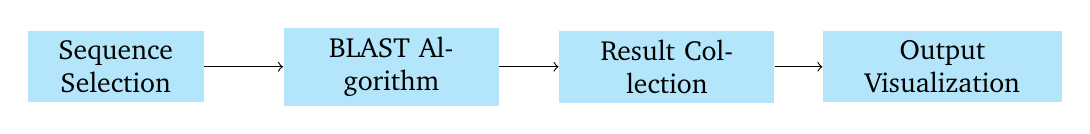
\begin{tikzpicture}[node distance=3.5cm, auto]
        \node (A) [fill=cyan!30,text width=2cm, align=center]{Sequence \\ Selection};;
        \node (B) [right of=A,fill=cyan!30,text width=2.5cm, align=center]{BLAST Algorithm};;
        \node (C) [right of=B,fill=cyan!30,text width=2.5cm, align=center]{Result Collection};;
        \node (D) [right of=C,fill=cyan!30,text width=2.8cm, align=center]{Output \\ Visualization};;
        \path[->] (A) edge (B);
        \path[->] (B) edge (C);
        \path[->] (C) edge (D);
    \end{tikzpicture}
    \caption{Basic working procedure of BLAST tool}
\end{figure}

\subsection{Sequence Selection}
A BLAST search requires two basic sequence- one which the search are going to be executed. One of them is the unknown sequence- it is referred as query sequence and, another is the database on which the tool is going to compare the sequences to. \\

During our BLAST search using the tool, we used Drosophila’s \textit{(Drosophila yakuba)} Mitochondrion DNA as our query sequence. And then the \textit{nt} database was selected as it contains the records of different nucleotide sequence.

\subsection{BLAST Algorithm}
The algorithm takes the input and database sequence, and then processed them using different methods. Finally, a scoring scheme is used to denote the similarity between sequences. In next chapter, the BLAST algorithm is going to be explained in detail.

\subsection{Result Collection}
The output result given by the NCBI BLAST API defaults in XML format. The BLAST tool returns the results along with other meta-data such as Hit Score/BLAST Score \footnote{The BLAST Score/Hit Score/Bit Score indicates the quality of the best alignment between the query sequence and the found sequence (hit). The higher the score, the better the alignment.}, E-value \footnote{E-value or ‘expect value’ is the number of matches by chance to the provided sequence one can expect in a database of a given size. Lower e values indicate more “significant” or better alignments.}, Query Range, Hit Range etc. \\

Formatted results are shown in the figure below- \\


\begin{figure}[H]
    \centering
    \verbinput{files/2_blast_result.txt}
    \caption{Result from NCBI BLAST API}
\end{figure}

\begin{figure}[H]
    \centering
    \verbinput{files/3_blast_hit_score.txt}
    \caption{BLAST Hit Score Output}
\end{figure}

\begin{figure}[H]
    \centering
    \verbinput{files/4_blast_hsp.txt}
    \caption{HSP Score}
\end{figure}

\subsection{Output Visualization}

The output result produced by the BLAST tool are most of them incomprehensible. Since the search is executed upon hundreds and thousands of different database sequences, it becomes hard to get an understanding of the alignment matching. Hence, the tool visualizes the output in a graphical manner which helps a user to identify most matching sequences. \\

The BLAST tool identifies different matching scores with individual colors so that it becomes easy to identify the regions. The following figure shows the output produced by the BLAST tool.

\begin{figure}[H]
    \centering
    \includegraphics[width=\textwidth]{files/visual_output.pdf}
    \caption{Output Visualization of a BLAST search}
\end{figure}

\chapter{BLAST Algorithm}
In this chapter, we are going to describe the BLAST algorithm with the help of an example. 

\section{Basic Terminologies}
\subsection{Numeric Representation of Sequences}

Bioinformatics algorithms, such as BLAST uses numerical representation to identify each sequences uniquely. The BLAST algorithm uses a \textbf{Base 4 Numeric Representation} to identify each unique nucleotide sequence by assigning each character in the sequence with a unique value. In the following table, numerical representation for the four nucleotides of DNA are shown.

\begin{table}[H]
    \centering
    \begin{tabular}{|c|c|c|}
        \hline
        Nucleotide  & Letter & Value \\\hline
        Adenine     & A      & 0     \\\hline
        Cytosine    & C      & 1     \\\hline
        Guanine     & G      & 2     \\\hline
        Thymine     & T      & 3     \\\hline
    \end{tabular}
    \caption{Numeric Representation of Nucleotides}
\end{table}

\subsection{K-mer Construction}
In \textbf{Bioinformatics}, k-mers are substrings of length $k$ contained within a biological sequence. Primarily used within the context of computational genomics and sequence analysis. \\

A sequence of length $L$ will have $L-k+1$ k-mers and $n^k$ total possible k-mers, where $n$ is number of possible monomers. For example, all the possible k-mers of a DNA sequence (\textbf{GTAGAGCTGT}) are shown below:

\begin{table}[H]
    \centering
    \renewcommand{\arraystretch}{1.4}
    \begin{tabular}{|c|l|}
        \hline
        \textbf{k}   &   \textbf{k-mers} \\\hline
        1   &   G, T, A, G, A, G, C, T, G, T    \\\hline
        2	&   GT, TA, AG, GA, AG, GC, CT, TG, GT  \\\hline
        3	&   GTA, TAG, AGA, GAG, AGC, GCT, CTG, TGT  \\\hline
        4	&   GTAG, TAGA, AGAG, GAGC, AGCT, GCTG, CTGT    \\\hline
        5	&   GTAGA, TAGAG, AGAGC, GAGCT, AGCTG, GCTGT    \\\hline
        6	&   GTAGAG, TAGAGC, AGAGCT, GAGCTG, AGCTGT  \\\hline
        7	&   GTAGAGC, TAGAGCT, AGAGCTG, GAGCTGT  \\\hline
        8	&   GTAGAGCT, TAGAGCTG, AGAGCTGT    \\\hline
        9	&   GTAGAGCTG, TAGAGCTGT    \\\hline
        10	&   GTAGAGCTGT  \\\hline
    \end{tabular}
    \caption{Different k-mers of the sequence \textit{GTAGAGCTGT}}
\end{table}

\section{Pre-processing of Database}

\subsection{Constructing 3-mers}
We select GGACGGATTCC  as a database sequence. Now we need to construct the 3-mers and calculate the position and key values of them. Duplicate 3-mers should be avoided and base 4 representation of the 3-mers should be selected as their key values. Then the obtained table is sorted with respect to the key value. \\
    \begin{table}[h]
        \centering
        \renewcommand{\arraystretch}{1}
        \begin{tabular}{c c c c}
             \begin{tabular}{| c | c | c |}
                \hline
                3-mers  &  Position & Key  \\ 
                \hline
                GGA &   1,5 &   40 \\
                \hline
                GAC &   2 &   33 \\
                \hline
                ACG &   3 &   6 \\
                \hline
                CGG &   4 &   26 \\
                \hline
                GAT &   6 &   35 \\
                \hline
                ATT &   7 &   15 \\
                \hline
                TTC &   8 &   61 \\
                \hline
                TCC &   9 &   53 \\
                \hline
            \end{tabular} & & & \begin{tabular}{| c | c | c |}
                \hline
                3-mers  &  Position & Key  \\ 
                \hline
                ACG &   3 &   6 \\
                \hline
                ATT &   7 &   15 \\
                \hline
                CGG &   4 &   26 \\
                \hline
                GAC &   2 &   33 \\
                \hline
                GAT &   6 &   35 \\
                \hline
                GGA &   1,5 &   40 \\
                \hline
                TCC &   9 &   53 \\
                \hline
                TTC &   8 &   61 \\
                \hline
            \end{tabular} \\
             
        \end{tabular}
        \caption{ (a) Generated 3-mers   (b) Sorted 3-mers with respect to key values}
        \label{tab:1}
    \end{table}
    
\newpage
    
\subsection{Building Binary Search Tree}

Now we are going to construct a binary search tree. We select the positions and keys of the 3-mers as nodes. \\
    \begin{figure}[h]
     \centering
        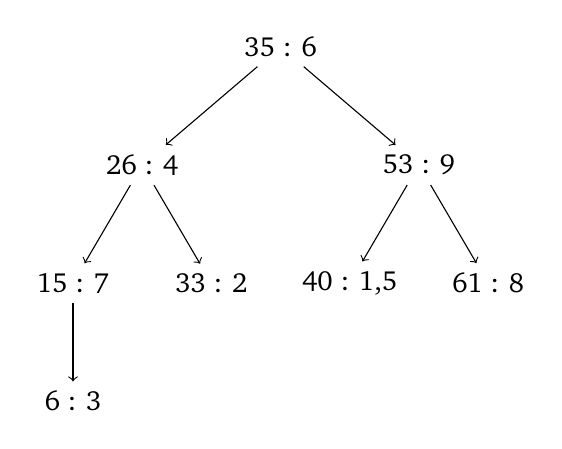
\begin{tikzpicture}[->, level/.style={
                                    sibling distance=2cm,
                                    level distance=1.5cm,
                                    level 1/.style={sibling distance=10em},
                                    level 2/.style={sibling distance=5em},
                                    level 3/.style={sibling distance=5em}
                                }
                            ]
            
            \node{35 : 6}
                child {node{26 : 4}
                    child {node{15 : 7}
                        child {node{6 : 3}}
                    }
                    child {node{33 : 2}}
                }
                child {node{53 : 9}
                    child {node{40 : 1,5}}
                    child {node{61 : 8}}
            };
        \end{tikzpicture}
        \caption{Constructed binary search tree}
        \label{fig:Tree}
    \end{figure}
    
With this, our pre-processing of the database sequence is done. Now we proceed to the next step.            

\section{Construction of k-mers From Query Sequence}
First of all, we should consider the following table representing the scoring scheme. \\
\begin{table} [h]
    \centering
    \renewcommand{\arraystretch}{1.4}
    \begin{tabular}{ | c | c | }
        \hline
        \multicolumn{2}{| c |}{Scoring Scheme}  \\ 
        \hline
        Match           &   1 \\
        \hline
        Mismatch        &  -1 \\
        \hline
        Gap Insertion   &   -1 \\
        \hline
        HSP Threshold   &   1 \\
        \hline
    \end{tabular}
    \caption{ Scoring Scheme}
        \label{tab:2}
\end{table}
\newpage
Let us consider ATCG as a query sequence. The 3-mers of this sequence are ATC and TCG. \\

\begin{table} [h]
    \centering
    \renewcommand{\arraystretch}{1}
    \begin{tabular}{ c c c c }
        \begin{tabular}{| c | c |}
                            \hline
                            3-mers  & Key  \\ 
                            \hline
                            ATC &   13 \\
                            \hline
                            CTC &   45 \\
                            \hline
                            GTC &   49 \\
                            \hline
                            TTC &   61 \\
                            \hline
                            AAC &   1 \\
                            \hline
                            ACC &   5 \\
                            \hline
                            AGC &   9 \\
                            \hline
                            ATA &   12 \\
                            \hline
                            ATG &   14 \\
                            \hline
                            ATT &   15 \\
                            \hline
                        \end{tabular} & & & \begin{tabular}{| c | c |}
                            \hline
                            3-mers  & Key  \\ 
                            \hline
                            TCG &   54 \\
                            \hline
                            ACG &   6 \\
                            \hline
                            CCG &   24 \\
                            \hline
                            GCG &   38 \\
                            \hline
                            TAG &   50 \\
                            \hline
                            TGG &   58 \\
                            \hline
                            TTG &   62 \\
                            \hline
                            TCA &   52 \\
                            \hline
                            TCC &   53 \\
                            \hline
                            TCT &   59 \\
                            \hline
                        \end{tabular}
    \end{tabular}
    \caption{ Selected K-mers with minimum HSP threshold}
    \label{tab:3}
\end{table}

Here we compare all possible 3-mers with the query 3-mers and select those whose matching score is at least the defined value of HSP threshold. We also calculate the key values of these 3-mers.\\

\section{Comparing k-mer with Pre-processed Data}

In this section, we are going to search the key value of the selected 3-mers with minimum HSP threshold in tree \ref{fig:Tree}. \\

\begin{figure}[h]
\begin{floatrow}
\capbtabbox{%
  \begin{tabular}{| c | c | c |}
            \hline
            3-mers  &  Position & Key  \\ 
            \hline
            ACG &   3 &   6 \\
            \hline
            ATT &   7 &   15 \\
            \hline
            CGG &   4 &   26 \\
            \hline
            GAC &   2 &   33 \\
            \hline
            GAT &   6 &   35 \\
            \hline
            GGA &   1,5 &   40 \\
            \hline
            TCC &   9 &   53 \\
            \hline
            TTC &   8 &   61 \\
            \hline
        \end{tabular}
}{%
  \caption{3-mers of Database Sequence}%
}
\ffigbox{%
  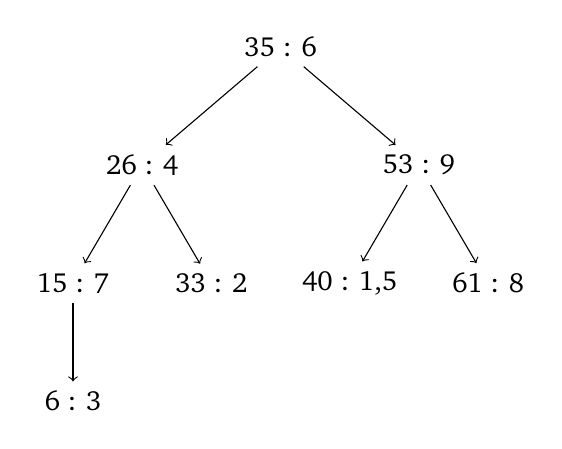
\begin{tikzpicture}[->, level/.style={
                                sibling distance=2cm,
                                level distance=1.5cm,
                                level 1/.style={sibling distance=10em},
                                level 2/.style={sibling distance=5em},
                                level 3/.style={sibling distance=5em}
                            }
                        ]
        
            \node{35 : 6}
                child {node{26 : 4}
                    child {node{15 : 7}
                        child {node{6 : 3}}
                    }
                    child {node{33 : 2}}
                }
                child {node{53 : 9}
                    child {node{40 : 1,5}}
                    child {node{61 : 8}}
            };
        \end{tikzpicture}
}{%
  \caption{Constructed binary search tree}%
}

\end{floatrow}
\end{figure}
\newpage
The 1st key found in the bst is 61. Its position is 8 and the corresponding 3-mer is TTC. \\

\begin{figure}[h]
\begin{floatrow}
\capbtabbox{%
  \begin{tabular}{ c c c c c}
        \begin{tabular}{| c | c |}
                            \hline
                            3-mers  & Key  \\ 
                            \hline
                            ATC &   13 \\
                            \hline
                            CTC &   45 \\
                            \hline
                            GTC &   49 \\
                            \hline
                            \cellcolor[HTML]{AFEEEE}{\color[HTML]{000000} TTC} &   \cellcolor[HTML]{AFEEEE}{\color[HTML]{000000} 61} \\
                            \hline
                            AAC &   1 \\
                            \hline
                            ACC &   5 \\
                            \hline
                            AGC &   9 \\
                            \hline
                            ATA &   12 \\
                            \hline
                            ATG &   14 \\
                            \hline
                            ATT &   15 \\
                            \hline
                        \end{tabular} & & \begin{tabular}{| c | c |}
                            \hline
                            3-mers  & Key  \\ 
                            \hline
                            TCG &   54 \\
                            \hline
                            ACG &   6 \\
                            \hline
                            CCG &   24 \\
                            \hline
                            GCG &   38 \\
                            \hline
                            TAG &   50 \\
                            \hline
                            TGG &   58 \\
                            \hline
                            TTG &   62 \\
                            \hline
                            TCA &   52 \\
                            \hline
                            TCC &   53 \\
                            \hline
                            TCT &   59 \\
                            \hline
                        \end{tabular} & &
    \end{tabular}
}{%
  \caption{3-mers with Minimum HSP Value}%
}

\capbtabbox{%
  \begin{tabular}{| c | c | c |}
            \hline
            3-mers  &  Position & Key  \\ 
            \hline
            ACG &   3 &   6 \\
            \hline
            ATT &   7 &   15 \\
            \hline
            CGG &   4 &   26 \\
            \hline
            GAC &   2 &   33 \\
            \hline
            GAT &   6 &   35 \\
            \hline
            GGA &   1,5 &   40 \\
            \hline
            TCC &   9 &   53 \\
            \hline
            \cellcolor[HTML]{AFEEEE}{\color[HTML]{000000} TTC} &
            \cellcolor[HTML]{AFEEEE}{\color[HTML]{000000} 8} &            \cellcolor[HTML]{AFEEEE}{\color[HTML]{000000} 61} \\
            \hline
        \end{tabular}
}{%
  \caption{3-mers of Database Sequence}%
}
\end{floatrow}
\end{figure}

 \begin{figure}[h]
     \centering
        \begin{tikzpicture}[->, level/.style={
                                    sibling distance=2cm,
                                    level distance=1.5cm,
                                    level 1/.style={sibling distance=10em},
                                    level 2/.style={sibling distance=5em},
                                    level 3/.style={sibling distance=5em}
                                }
                            ]
            
            \node{35 : 6}
                child {node{26 : 4}
                    child {node{15 : 7}
                        child {node{6 : 3}}
                    }
                    child {node{33 : 2}}
                }
                child {node{53 : 9}
                    child {node{40 : 1,5}}
                    child {node[normal]{61 : 8}}
            };
        \end{tikzpicture}
        \caption{Constructed binary search tree}
        \label{fig:Tree}
    \end{figure}

Following the similar process we have found 15, 6 and 53. The corresponding (3-mers, position) pairs are \textbf{(ATT, 7)}, \textbf{(ACG, 3)} and \textbf{(TCC, 9)} respectively. \\

\section{Alignment Extension}

\subsection{Seeding}
The next step is seeding. Seeding means finding exact matches of the part of the database with the part of the query. For 3-mers ACG, ATT, TTC and TCC, the starting position to put 3 consecutive crosses are 3, 7, 8 and 9 respectively. \\ 
\newpage
\begin{table}[h]
    \centering
    \begin{tabular}{| c | c | c | c | c | c | c | c | c | c | c | c |}
        \hline
         & G & G & A & C   &   G   &   G   &   A   &   T   &   T   &   C   &   C  \\
        \hline
        A &  &   &  &   &  &   &   X   &   X   &    &   &   \\
        \hline
        T &  &   & X &   &  &   &   &   X   & X   &   &   \\
        \hline
        C &  &   &  & X  &  &   &    &   &  X  & X  &   \\
        \hline
        G &  &   &  &   & X &   &    &    &    &   &  X \\
        \hline
    \end{tabular}
    \caption{Seeding}
    \label{tab:4}
\end{table}
Now we are going to apply the \textbf{Smith-Waterman Algorithm} to determine the extension of the local alignments.. \\
\subsection{Extension of the Seeding}
 After applying the algorithm we obtain the following table. Now we are going to extend the alignments. Recall that, the score extension threshold was 1. \\
 
\begin{table}[h]
    \centering
    \renewcommand{\arraystretch}{1}
    
    \begin{tabular}{| c | c | c | c | c | c | c | c | c | c | c | c | c |}
        \hline
        & - & G & G & A & C   &   G   &   G   &   A   &   T   &   T   &   C   &   C  \\
        \hline
        - & &  &  &  &   &   &   &    &     &    &     &    \\
        \hline
        A & &  &   &  &   &  &   &  1  &    &    &   &   \\
        \hline
        T & & &   &  &   &  &   &   &   2  & 1  &   &   \\
        \hline
        C &  & &   &  & 1  &  &   &    &  1 &  1 & 2  &  1 \\
        \hline
        G &  & &  &  &   & 2 &  1 &    &    &    &  1 &  1 \\
        \hline
    \end{tabular}
    \caption{Extension of alignment}
    \label{tab:5}
\end{table}

This first local alignment found from the table is in table \ref{tab:6} . The upper segment is from the database sequence and the lower segment is from the query sequence. \\

\begin{figure}[h]
\begin{floatrow}
\capbtabbox{%
  \begin{tabular}{c c  c  c  c c c }
           & & C & G & G & & \\
           & & C & G & - & & \\
        \end{tabular}
}{%
  \caption{Alignments}
  \label{tab:6}%
}
\capbtabbox{%
  \begin{tabular}{| c | c | c | c | c | c | c | c | c | c | c | c | c |}
                \hline
                & - & G & G & A & C   &   G   &   G   &   A   &   T   &   T   &   C   &   C  \\
                \hline
                - & &  &  &  &   &   &   &    &     &    &     &    \\
                \hline
                A & &  &   &  &   &  &   &  1  &    &    &   &   \\
                \hline
                T & & &   &  &   &  &   &   &   2  & 1  &   &   \\
                \hline
                C &  & &   &  &  \cellcolor[HTML]{AFEEEE}{\color[HTML]{000000} 1}  &  &   &    &  1 &  1 & 2  &  1 \\
                \hline
                G &  & &  &  &   &\cellcolor[HTML]{AFEEEE}{\color[HTML]{000000} 2} &  \cellcolor[HTML]{AFEEEE}{\color[HTML]{000000} 1} &    &    &    &  1 &  1 \\
                \hline
            \end{tabular}
}{%
  \caption{3-mers of Database Sequence}%
}
\end{floatrow}
\end{figure}
\newpage

Following the same approach, we get 6 local alignments. \\

\begin{figure}[h]
\begin{floatrow}
\capbtabbox{%
  \begin{tabular}{ c  c  c c c }
            C & G & G & & \\
            C & G & - & & \\
            & & & & \\
            A & T & T & & \\
            A & T & C & & \\
            & & & & \\
            A & T & - & & \\
            A & T & C & & \\
        \end{tabular}
}{
}
\capbtabbox{%
  \begin{tabular}{ c c c  c  c c c }
             &  & A & T & T & C & C \\
             &  & A & T & - & C & G \\
             & & & & & & \\
             &  & A & T & T & C & C \\
             &  & A & T & - & C & - \\
             & & & & & & \\
             &  & A & T & T & C & - \\
             &  & A & T & - & C & G \\
        \end{tabular}
}{
}
\end{floatrow}
\end{figure}

\section{Complexity of the Algorithm}
In this section, we are going to determine the complexity of the BLAST algorithm. The number of k-mers in a $X$ length string can be expressed as $X-K+1$ where $K$ is the length of a k-mer. So the number of k-mers in the $M$ length database sequence and the number of k-mers in the $L$ length query sequence is calculated below. \\ 

$M$ length Database, 
\begin{equation}
n_{k-mer} = M - K + 1
\end{equation}

$L$ length Query,
\begin{equation}
n_{k-mer} = L - K + 1
\end{equation}

As we have used the binary search tree to find the k-mers, the complexity of the algorithm is, $$\mathcal{O}(\{L-K+1\}\times\log_{2}\{M-K+1\})$$ Here, K = k-mer length, L = Length of query sequence and M = Total length of database sequences. \\
Since $K$ is constant, we can express the complexity as, $$\mathcal{O}(L\times\log_{2}M)$$


\chapter{Conclusion}
BLAST is a powerful tool for finding local alignments. Since BLAST uses \textbf{Smith Waterman Algorithm} to extend the local alignments, other methods can also be used in place in order to increase the efficiency of the overall process. FASTA, the predecessor to BLAST is however slower than BLAST but produces exact matches through a much wider range of scoring matrices, making it easier to tailor a search to a specific single sequence. On the other hand, an extremely fast but less sensitive alternative to BLAST is BLAT (Blast Like Alignment Tool). \\

The BLAST approach allows extremely fast approach to search database and to match and extend the alignments. BLAST is more time-efficient than FASTA by searching only for the more significant patterns in the sequences, yet with comparative sensitivity. This is what makes BLAST more convenient than other existing algorithms of the same kind.

\chapter*{References}
\addcontentsline{toc}{chapter}{References}  

\begin{enumerate}

    \item {\small Altschul, S. F., et al. “Basic Local Alignment Search Tool.” Journal of Molecular Biology, vol. 215, no. 3, Oct. 1990, pp. 403–10. PubMed, doi:10.1016/S0022-2836(05)80360-2.}
    
    \item {\small Smith, T. F., and M. S. Waterman. “Identification of Common Molecular Subsequences.” Journal of Molecular Biology, vol. 147, no. 1, Mar. 1981, pp. 195–97. DOI.org (Crossref), doi:10.1016/0022-2836(81)90087-5.}
    
    \item {\small BLAST: Basic Local Alignment Search Tool. https://blast.ncbi.nlm.nih.gov/Blast.cgi. Accessed 12 July 2021.}
    
    \item {\small GitHub - NCBI-Hackathons/NCBIComputationalCookbook: Jupyter Notebooks to More Effectively Leverage Computational Resources at NCBI.” GitHub, https://github.com/NCBI-Hackathons/NCBIComputationalCookbook. Accessed 28 July 2021.}
    
    \item {\small PR-INBRE BiRC [Bioinformatics Resources Core] - YouTube. \\ https://www.youtube.com/channel/UC8kHK9I5NxHmW0j-RcWQ8cg. Accessed 12 July 2021.}
    
    \item {\small Index of /Blast/Db. https://ftp.ncbi.nlm.nih.gov/blast/db/. Accessed 28 July 2021.}
\end{enumerate}

\end{document}
